% Provenance (never printed): see sources/outline_sources.md (Year 3: the main
% field and its secular variation, rock magnetism, palaeomagnetic poles, apparent
% polar wander, magnetostratigraphy, the geodynamo). Brief: sources/book5/BRIEFS.md,
% ch. 4. Curves and maps from figdata/bachelor-3/igrf_field.py (IGRF-14),
% palaeomag_stats.py (the invented Kesta terrane, its Fisher statistics, the
% Zijderveld specimen and the reference APW path), magnetostratigraphy.py.
% Exercise and problem values in the Book 5 scratch calculator calc/ch04.py.
\chapter{المغناطيسية الأرضية والمغناطيسية القديمة}\label{ch:b3:palaeomagnetism}

تدفّقٌ بازلتيّ ثار قبل ستين مليون سنة، فبرد وحبيباتُ المغنتيت الدقيقة فيه
محبوسةٌ موازيةً لمجال ذلك الزمن. يُثقب اليوم ويُوجَّه في
موضعه، ويُقطَّع إلى أسطوانات صغيرة، ويُسخَّن
خطوةً خطوةً في غرفةٍ معزولةٍ عن المجال الحالي، فإنّه ما يزال يدلّ على مدى بُعده
آنذاك عن القطب، وعلى الجهة التي كان يواجهها. آلاف من هذه
القياسات، من كل قارّة وكل عصر، بيّنت كيف تحرّكت القارّات
قبل أن تتكوّن قيعان المحيطات التي تسجّل حركتها، وفي أيّ
ترتيبٍ انعكس فيه المجال عبر طبقات
مقطعٍ رسوبيّ. يصف هذا الفصل المجال كما هو اليوم، وكيف تسجّله الصخور،
كيف يُستخلص اتجاهٌ ويُحسب متوسطه، وماذا يقول القطب المغناطيسي القديم
عن حركة صفيحة.

\begin{recall}
الأرض بوصفها مغناطيسًا والانحراف المغناطيسي وردا في كتب الفيزياء
المدرسية؛ النطاقات المغناطيسية والتخلّف المغناطيسي والمغنطة المتبقية ودرجة حرارة كوري
في مجلد السنة الثالثة؛ ومجال ثنائي القطب المغناطيسي في
مجلد السنة الأولى. وقد عُرضت الانعكاسات المغناطيسية والقطبيتان العادية والمعكوسة
في الصف 11. وعُرِّفت الدائرة العظمى والمثلّث الكروي في
مجلد السنة الأولى، في فصله عن الفلك الكروي؛ والحقبة القطبية،
والمقياس الزمني لقطبية المجال المغناطيسي الأرضي، والشذوذ المغناطيسي البحري، والدورانات المنتهية
حول قطب أويلر في فصله عن حركيات الصفائح على الكرة؛
ومسار البقعة الساخنة في فصله عن البقع الساخنة. والتوافقيات الكروية
ودوال ليجندر المعيارية وفق شميدت $P_n^m$ استُخدمت للجاذبية في
الفصل عن الجاذبية وشكل الأرض (\cref{ch:b3:gravity-geodesy}).
\end{recall}

\section{المجال الرئيسي}

\begin{definition}[المجال المغناطيسي الأرضي الرئيسي؛ ثنائي القطب المحوري المركزي الأرضي]\label{def:b3:palaeomagnetism:main-field}
\emph{المجال المغناطيسي الأرضي الرئيسي}\index{المجال المغناطيسي الأرضي الرئيسي} هو الجزء من
المجال المغناطيسي للأرض الناشئ داخلها، في لبّها الخارجي السائل المكوّن من الحديد؛
يتغيّر خلال سنوات حتى ملايين السنين، على خلاف مجالي الغلاف الأيوني
والغلاف المغناطيسي، اللذين يتغيّران خلال ثوانٍ إلى أيام. أمّا
\emph{ثنائي القطب المحوري المركزي الأرضي}\index{ثنائي القطب المحوري المركزي الأرضي} فهو مجال ثنائي قطب مغناطيسي موضوع
في مركز الأرض ومحاذٍ لمحور دورانها،
موجّهًا نحو الجنوب، بحيث تخرج خطوط مجاله من نصف الكرة الجنوبي
وتدخل إلى نصف الكرة الشمالي.
\end{definition}

عند أيّ نقطة من السطح، المجال $\mathbf F$ متجهةٌ. ويُوصَف في إطار محلي (انظر الشكل أدناه):
$X$ نحو الشمال الجغرافي، و$Y$ نحو الشرق،
و$Z$ نحو الأسفل. مركبته الأفقية هي $H = \sqrt{X^2 + Y^2}$، وشدّته
الكلية $F = |\mathbf F|$، والانحراف المغناطيسي $D$ هو الزاوية من
الشمال الجغرافي إلى $\mathbf H$ مقيسةً في اتجاه عقارب الساعة، \omterm{def:b3:palaeomagnetism:inclination}{والميل المغناطيسي} $I$
هو الزاوية من الأفق إلى $\mathbf F$.

\begin{definition}[الميل المغناطيسي]\label{def:b3:palaeomagnetism:inclination}
\emph{الميل المغناطيسي}\index{الميل المغناطيسي} $I$ للمجال عند
نقطةٍ ما هي الزاوية بين متجهة المجال والمستوى الأفقي،
موجبةً عندما يتّجه المجال نحو الأسفل: $\tan I = Z/H$، مع $-\ang{90} \le I
\le \ang{90}$.
\end{definition}

\begin{omfigure}
\begin{tikzpicture}[font=\small, x=1cm, y=1cm, >={Stealth[length=5pt]}]
% schematic; X = 3.0, Y = 1.0 (along the oblique east axis), Z = 2.4
\coordinate (O) at (0,0);
\coordinate (E) at (0.9,0.65);
\fill[gray!12] (-0.6,-0.43) -- (3.6,-0.43) -- ($(3.6,-0.43)+2.2*(E)$) -- ($(-0.6,-0.43)+2.2*(E)$) -- cycle;
\draw[->] (O) -- (4.0,0) node[right] {\foreignlanguage{arabic}{\mbox{\textdir TLT $X$}، الشمال الجغرافي}};
\draw[->] (O) -- ($1.9*(E)$) node[above right] {\foreignlanguage{arabic}{\mbox{\textdir TLT $Y$}، الشرق}};
\draw[->] (O) -- (0,-3.0) node[below] {\foreignlanguage{arabic}{\mbox{\textdir TLT $Z$}، نحو الأسفل}};
\coordinate (Hh) at ($(3.0,0)+1.0*(E)$);
\coordinate (F) at ($(Hh)+(0,-2.4)$);
\draw[densely dashed, gray] (3.0,0) -- (Hh);
\draw[densely dashed, gray] ($1.0*(E)$) -- (Hh);
\draw[densely dashed, gray] (Hh) -- (F);
\draw[densely dashed, gray] (0,-2.4) -- (F);
\draw[very thick, ->, blue!60!black] (O) -- (Hh) node[pos=0.3, above, sloped] {$\mathbf H$};
\draw[very thick, ->, red!70!black] (O) -- (F) node[pos=0.55, below left] {$\mathbf F$};
\draw[thick] (1.25,0) arc[start angle=0, end angle=9.46, radius=1.25];
\node at (1.62,0.13) {$D$};
\draw[thick, red!70!black] ($0.36*(Hh)$) to[bend left=30] ($0.3*(F)$);
\node[red!70!black] at (1.62,-0.42) {$I$};
\end{tikzpicture}

\par\smallskip{\small عناصر المجال عند نقطة: المركبات الشمالية $X$ والشرقية
$Y$ والمركبة نحو الأسفل $Z$، والمركبة الأفقية $\mathbf H$، والمجال الكلي
$\mathbf F$، والانحراف المغناطيسي $D$ (في المستوى الأفقي، باللون الرمادي)
\omterm{def:b3:palaeomagnetism:inclination}{والميل المغناطيسي} $I$ (في المستوى الرأسي الذي يحتوي $\mathbf
F$).}\label{fig:b3:palaeomagnetism:elements}
\end{omfigure}

\begin{theorem}[صيغة ثنائي القطب]\label{thm:b3:palaeomagnetism:dipole}
عند سطح كرة نصف قطرها $a$، لمجال \omterm{def:b3:palaeomagnetism:main-field}{ثنائي القطب المحوري المركزي الأرضي}
ذي العزم $m$ له عند خط العرض $\lambda$ القيم الآتية:
\[
  H = B_0\cos\lambda,\qquad Z = 2B_0\sin\lambda,\qquad
  F = B_0\sqrt{1 + 3\sin^2\lambda},\qquad
  \tan I = 2\tan\lambda,\qquad D = 0,
\]
حيث $B_0 = \mu_0 m/(4\pi a^3)$ هو المجال عند خط الاستواء. وهذه هي
\emph{صيغة ثنائي القطب}\index{صيغة ثنائي القطب}.
\end{theorem}

\begin{proof}
خارج مصادره يُشتقّ المجال من كمونٍ سلّمي مغناطيسي،
$\mathbf B = -\nabla V$. بالنسبة إلى ثنائي قطب عزمه $m$ موجّه على طول $-z$،
أي نحو الجنوب الجغرافي، $V = -\mu_0 m\cos\theta/(4\pi r^2)$، حيث $\theta$
متمّم خط العرض. في الإحداثيات الكروية، $B_r = -\partial V/\partial r =
-2\mu_0 m\cos\theta/(4\pi r^3)$ و$B_\theta = -(1/r)\,\partial V/\partial\theta =
-\mu_0 m\sin\theta/(4\pi r^3)$، و$B_\varphi = 0$. عند $r = a$، تكون المركبة نحو الأسفل
هي $Z = -B_r = 2B_0\cos\theta = 2B_0\sin\lambda$، ولأنّ
$\mathbf e_\theta$ يشير نحو الجنوب، فإنّ المركبة الشمالية هي $X = -B_\theta =
B_0\sin\theta = B_0\cos\lambda$، مع $Y = 0$. إذن $H = X$، و$D = 0$، و$\tan I =
Z/H = 2\tan\lambda$ و$F^2 = B_0^2(\cos^2\lambda + 4\sin^2\lambda) =
B_0^2(1 + 3\sin^2\lambda)$.
\end{proof}

يكون الميل صفرًا عند خط الاستواء، و\ang{90} عند القطب الشمالي،
وسالبًا في نصف الكرة الجنوبي؛ وتكون الشدّة ضعف قيمتها عند القطبين مقارنةً
بخط الاستواء. المجال الحقيقي ليس ثنائي قطب مثاليًا، ويُوصف،
كما هو الحال مع الجاذبية، بالتوافقيات الكروية.

\begin{definition}[المجال المغناطيسي الأرضي المرجعي الدولي]\label{def:b3:palaeomagnetism:igrf}
\emph{المجال المغناطيسي الأرضي المرجعي الدولي}\index{المجال المغناطيسي الأرضي المرجعي الدولي}
(IGRF) هو النموذج المتفق عليه دوليًا للمجال
الرئيسي: الكمون، على السطح وفوقه،
\[
  V(r,\theta,\varphi) = a\sum_{n=1}^{N}\Bigl(\frac ar\Bigr)^{n+1}\sum_{m=0}^{n}
  \bigl(g_n^m\cos m\varphi + h_n^m\sin m\varphi\bigr)P_n^m(\cos\theta),
\]
حيث $a = \qty{6371.2}{km}$، و$\mathbf B = -\nabla V$، ومعاملات غاوس
$g_n^m$، $h_n^m$ (بوحدة \unit{nT}) تُعطى كل خمس سنوات منذ 1900،
مع معدّل تغيّرها خلال الخمس سنوات التالية.
\end{definition}
% ledger: geomag5:igrf, data:b5-igrf

يُصان النموذج من قِبل الجمعية الدولية للمغناطيسية وفيزياء
الغلاف العلوي؛ وقد اكتمل جيله الرابع عشر في تشرين الثاني/نوفمبر 2024، ويُقتصر على
الدرجة $N = 13$. الحد الأول، $g_1^0$، هو ثنائي القطب المحوري:
وبالمقارنة مع البرهان أعلاه، $B_0 = -g_1^0$، و$g_1^0 = \qty{-29350}{nT}$
في عام 2025. ومع الحدّين الآخرين من الدرجة الأولى يكون ثنائي القطب مائلًا؛ ويلتقي محوره
بالسطح عند القطب المغناطيسي الأرضي الشمالي، عند \ang{80.79}\,شمالًا، \ang{72.76}\,غربًا في
عام 2025، وعزمه $m = 4\pi a^3\sqrt{(g_1^0)^2 + (g_1^1)^2 +
(h_1^1)^2}/\mu_0 = \qty{7.69e22}{A.m^2}$.
% ledger: data:b5-igrf

\begin{omfigure}
\begin{tikzpicture}
\begin{groupplot}[group style={group size=1 by 2, vertical sep=1.4cm},
  ommap, width=0.96\linewidth, xtick={-180,-120,...,180}, ytick={-60,0,60},
  unbounded coords=jump, title style={font=\small, yshift=-1ex}]
\nextgroupplot[title={(أ) الميل، كل \ang{20}}]
% computed in figdata/bachelor-3/igrf_field.py; ledger: data:b5-igrf, data:ne-land
\addplot[fill=omLithAlluv, draw=black!45, line width=0.2pt, forget plot] table {figdata/out/shared-geo-land.dat};
\addplot[red!70!black, line width=0.5pt] table[x=x, y=y] {figdata/out/bachelor-3-igrf_field-incl.dat};
\addplot[black, line width=1.1pt] table[x=x, y=y] {figdata/out/bachelor-3-igrf_field-dipeq.dat};
\addplot[draw=none, nodes near coords, point meta=explicit,
  every node near coord/.style={font=\tiny, fill=white, inner sep=0.6pt, anchor=center}]
  table[x=x, y=y, meta=lev] {figdata/out/bachelor-3-igrf_field-inclab.dat};
\nextgroupplot[title={(ب) الشدّة الكلّية، كل \qty{5000}{nT}}]
\addplot[fill=omLithAlluv, draw=black!45, line width=0.2pt, forget plot] table {figdata/out/shared-geo-land.dat};
\addplot[blue!60!black, line width=0.5pt] table[x=x, y=y] {figdata/out/bachelor-3-igrf_field-intens.dat};
\addplot[draw=none, nodes near coords, point meta=explicit,
  every node near coord/.style={font=\tiny, fill=white, inner sep=0.6pt, anchor=center}]
  table[x=x, y=y, meta=lev] {figdata/out/bachelor-3-igrf_field-intlab.dat};
\addplot[only marks, mark=x, mark size=3pt, line width=1pt, black] table {figdata/out/bachelor-3-igrf_field-fmin.dat};
\end{groupplot}
\end{tikzpicture}

\par\smallskip{\small المجال الرئيسي في عام 2025 من \omterm{def:b3:palaeomagnetism:igrf}{المجال المغناطيسي الأرضي المرجعي الدولي} الرابع عشر، عند
سطح الكرة ذات نصف القطر \qty{6371.2}{km}. (أ) الميل بالدرجات؛
الخطّ السميك، $I = 0$، هو خط الميل الصفري. (ب) الشدّة الكلّية بوحدة \unit{nT}؛
العلامة المتقاطعة تمثّل أضعف مجال، نحو \qty{22100}{nT}، فوق
جنوب الأطلسي، مقابل نحو \qty{66600}{nT} عند أقواها، جنوب
أستراليا.}\label{fig:b3:palaeomagnetism:igrf-maps}
\end{omfigure}

تُبيّن الخرائط أعلاه مدى ابتعاد المجال عن ثنائي القطب. يتحرّك خط الميل الصفري
حتى نحو \ang{12} بعيدًا عن خط الاستواء الجغرافي، وتتغيّر الشدّة،
التي كان ثنائي القطب سيجعلها منتظمة على طول الدائرة الموازية، بعامل قدره
ثلاثة، مع منخفض واسع فوق جنوب الأطلسي.
% ledger: data:b5-igrf

\begin{definition}[التغيّر القرني]\label{def:b3:palaeomagnetism:secular}
\emph{التغيّر القرني}\index{التغيّر القرني} هو التغيّر البطيء للمجال
الرئيسي مع الزمن، على مدى سنوات إلى قرون، ويُقاس بمعدّل تغيّر
معاملات غاوس أو عناصره عند موضع ما.
\end{definition}

خلال آخر 125 سنة انخفض عزم ثنائي القطب من
\qty{8.32e22}{A.m^2} إلى \qty{7.69e22}{A.m^2}، أي بنسبة \qty{7.6}{\percent}، وانتقل القطب
المغناطيسي الأرضي الشمالي من \ang{78.61}\,شمالًا، \ang{68.79}\,غربًا إلى موقعه الحالي
(الشكل أدناه)؛ و$g_1^0$ لا يزال يتزايد بمقدار \qty{12.6}{nT} في السنة،
وهذا إضعاف لثنائي القطب.
% ledger: data:b5-igrf

\begin{omfigure}
\begin{tikzpicture}
\begin{groupplot}[group style={group size=2 by 1, horizontal sep=1.7cm},
  omrecord, width=0.47\linewidth, height=0.4\linewidth, xmin=1895, xmax=2030,
  xtick={1900,1950,2000}, xticklabel style={/pgf/number format/1000 sep=},
  xlabel={السنة}]
\nextgroupplot[ylabel={عزم ثنائي القطب \babelsublr{(\qty{e22}{A.m^2})}}, ymin=7.6, ymax=8.4]
% computed in figdata/bachelor-3/igrf_field.py; ledger: data:b5-igrf
\addplot[omDef, thick, mark=*, mark size=1pt] table[x=year, y=M] {figdata/out/bachelor-3-igrf_field-dipole.dat};
\nextgroupplot[ylabel={خط عرض القطب \babelsublr{(\unit{\degree}\,N)}}, ymin=78, ymax=81.5]
\addplot[red!70!black, thick, mark=*, mark size=1pt] table[x=year, y=plat] {figdata/out/bachelor-3-igrf_field-dipole.dat};
\end{groupplot}
\end{tikzpicture}

\par\smallskip{\small جزء ثنائي القطب من المجال الرئيسي، من 1900 إلى 2025، كل خمس
سنوات، من \omterm{def:b3:palaeomagnetism:igrf}{المجال المغناطيسي الأرضي المرجعي الدولي}: عزمه (يسارًا) وخط عرض القطب المغناطيسي الأرضي الشمالي
(يمينًا).}\label{fig:b3:palaeomagnetism:dipole}
\end{omfigure}

من أين يأتي المجال؟ يُستبعد أن يكون المغناطيس الدائم هو المصدر: فدرجة
كيوري للمغنتيت نحو \qty{580}{\celsius}، وللهيماتيت
\qty{675}{\celsius}، ولبّ الأرض العميق أشدّ حرارةً بكثير من ذلك. يتجدّد
المجال باستمرار بحركة السائل الموصل للكهرباء في اللبّ
الخارجي.
% ledger: tarduno:curie

\begin{definition}[الدينامو الأرضي]\label{def:b3:palaeomagnetism:geodynamo}
\emph{الدينامو الأرضي}\index{الدينامو الأرضي} هو العملية ذاتية الاستدامة التي
يُحدِث بها الحمل في سبيكة الحديد السائلة الموصلة للكهرباء في اللبّ الخارجي،
المنحرفة بفعل دوران الأرض، تيارات كهربائية يحفظ مجالها المغناطيسي نفسه
في مواجهة الاضمحلال الأومي.
\end{definition}

\begin{proposition}[معادلة الحث]\label{prop:b3:palaeomagnetism:induction}
في موصل ذي انتشارية مغناطيسية $\eta = 1/(\mu_0\sigma)$ يتحرك بالسرعة
$\mathbf u$، يخضع المجال المغناطيسي للمعادلة
\[
  \frac{\partial\mathbf B}{\partial t} = \nabla\times(\mathbf u\times\mathbf B)
  + \eta\nabla^2\mathbf B .
\]
\end{proposition}
\admitted

يُطيل الحدّ الأول خطوط المجال التي يحملها السريان ويلويها، أمّا
الحدّ الثاني فيجعل المجال يضمحلّ، في جسم حجمه $L$، خلال زمن من مرتبة
$L^2/\eta$. يعمل الدينامو حين يُعيد السريان توليد المجال أسرع مما ينتشر بعيدًا.
تُعيد المحاكاة الحاسوبية لغلافٍ مائعٍ دوّارٍ يحدث فيه الحمل إنتاج
ثنائي القطب المحوري السائد وانقلابًا بين حين وآخر، غير أنّ
معادلاتُ \omterm{def:b3:palaeomagnetism:geodynamo}{الدينامو الأرضي} المقترنةُ بمعادلات السريان تتجاوز
نطاق هذا الكتاب. وإلى جانب الانقلابات الكاملة، يحفظ السجلّ أحداثًا أقصر.

\begin{definition}[الانحراف المغناطيسي العابر]\label{def:b3:palaeomagnetism:excursion}
\emph{الانحراف المغناطيسي العابر}\index{الانحراف المغناطيسي العابر} هو انحراف كبير
لاتّجاه المجال عن اتّجاه ثنائي القطب المحوري، حين يبتعد
القطبُ المغناطيسي الأرضي الافتراضي (انظر \cref{def:b3:palaeomagnetism:vgp}) بعيدًا عن القطب الجغرافي،
ثمّ يعود إلى القطبية الأصلية بدلًا من
أن يُتمّ انقلابًا.
\end{definition}

\section{كيف تسجّل الصخور المجال}

تحمل المعادن الحديدية المغناطيسية بالمعنى الواسع، وأهمّها المغنتيت في الصخور النارية،
والهيماتيت في الرواسب الحمراء مغنطةً متبقية. فوق درجة حرارة كوري الخاصة بها لا تكون للحبيبة
أيّ مغنطة؛ وتحتها تكون الحبيبة الصغيرة نطاقًا مغناطيسيًّا مفردًا يتقلّب عزمه
بين اتّجاهاتها السهلة بتنشيط حراري، بعد
زمن استرخاء
\[
  \tau = \frac1C\exp\Bigl(\frac{K V}{k_B T}\Bigr),
\]
حيث $K$ طاقةُ الاتّجاهية المغناطيسية لوحدة الحجم، و$V$ حجمُ الحبيبة
و$C$ عامل تردّد. وهذه قاعدة نيل للاسترخاء، نُسلّم بها هنا. ولأنّ
$\tau$ يتزايد أُسّيًّا مع انخفاض $T$، تعبر الحبيبة فترةً ضيقةً من درجات الحرارة
من التقلّب الحرّ إلى الاحتفاظ بعزمها لمدّة تبلغ مليارات
السنين.

\begin{definition}[درجة حرارة الحجب]\label{def:b3:palaeomagnetism:blocking}
\emph{درجة حرارة الحجب}\index{درجة حرارة الحجب} للحبيبة المغناطيسية
هي الدرجة التي يتجاوز دونها زمنُ استرخائها زمنَ
التجربة، فيبقى عزمها ثابتًا: عند التبريد عبرها تُسجّل الحبيبة
المجالَ؛ وعند التسخين عبرها في غياب المجال تفقد ذلك
التسجيلَ.
\end{definition}

\begin{definition}[المغنطة المتبقية الطبيعية والحرارية والفتاتية والكيميائية]\label{def:b3:palaeomagnetism:nrm}
\emph{المغنطة المتبقية الطبيعية}\index{المغنطة المتبقية الطبيعية}
(NRM) للصخر، وهي المغنطة المتبقية التي يحملها وقت جمعه، أي مجموع
المركّبات المكتسبة في أزمنة مختلفة. و\emph{المغنطة المتبقية
الحرارية}\index{المغنطة المتبقية الحرارية} (TRM) تُكتسب بالتبريد عبر
\omterm{def:b3:palaeomagnetism:blocking}{درجات الحجب} في مجال مغناطيسي، كما في جريان الحمم أو
جسم متداخل. و\emph{المغنطة المتبقية الفتاتية}\index{المغنطة المتبقية الفتاتية}
(DRM) تُكتسب حين تستقرّ حبيبات مغناطيسية في الماء، أو في
الرواسب الرطبة الواقعة تحت سطحها مباشرةً، فتدور نحو المجال قبل أن
تُحبَس. و\emph{المغنطة المتبقية الكيميائية}\index{المغنطة المتبقية الكيميائية}
(CRM) تُكتسب حين ينمو معدنٌ مغناطيسي، عبر
حجم حجب، في مجال، كما يحدث للهيماتيت عند تكوّن طبقة حمراء.
\end{definition}

يُسجّل TRM المجال لحظة التبريد، و DRM خلال الزمن الذي
يستغرقه الرسوب في التراصّ؛ و CRM فيُسجّل متى نما المعدن، وقد يكون ذلك بعيدًا
عن الترسيب. ويُضيف تسخينٌ لاحق، أو المجال الحالي المؤثّر زمنًا طويلًا
في حبيبات ذات زمن استرخاء قصير، مركّبةً ثانويةً تُضاف فوق ما سبق:
مغنطةً متبقيةً لزجةً على امتداد المجال الحديث.

\section{من العيّنة إلى الاتّجاه}

تُحفر أسطوانات موجَّهة في عدّة مواقع من التكوين، بضع أسطوانات في كلّ
موقع، وتُقطَّع إلى عيّنات حجمها بضعة سنتيمترات مكعّبة. تُقاس NRM لكلّ عيّنة،
ثمّ تُزال تدريجيًّا.

\begin{definition}[إزالة المغنطة المتدرّجة]\label{def:b3:palaeomagnetism:demag}
\emph{إزالة المغنطة المتدرّجة}\index{إزالة المغنطة المتدرّجة} هي إزالة
المغنطة المتبقية للعيّنة على خطوات متزايدة الشدّة، مع قياس المتجهة الباقية بعد
كلّ خطوة: بالتسخين إلى درجات متزايدة ثمّ بالتبريد
في غياب المجال (الإزالة الحرارية)، وهي تزيل المركّبات ذات درجة الحجب الأدنى أوّلًا،
أو بمجالات مغناطيسية متناوبة متزايدة القيمة القصوى،
تتناقص إلى الصفر (الإزالة بالمجال المتناوب)، وهي تزيل
تلك ذات القسرية الأدنى أوّلًا.
\end{definition}

\begin{definition}[مخطط زيجدرفيلد؛ المغنطة المتبقية المميِّزة]\label{def:b3:palaeomagnetism:zijderveld}
\emph{مخطط زيجدرفيلد}\index{مخطط زيجدرفيلد} يرسم نقاط نهاية
متجهة المغنطة المتبقية الباقية بعد كلّ خطوة من الإزالة، على مستويين معًا:
المستوي الأفقي (الشمال مقابل الشرق) ومستوٍ رأسي (الشمال مقابل الأسفل)،
بمحور شمالي مشترك. والمركّبة المُزالة وحدها عبر مدًى من
الخطوات تُرسم قطعةً مستقيمة؛ والقطعة المنتهية عند نقطة الأصل هي
\emph{المغنطة المتبقية المميِّزة}\index{المغنطة المتبقية المميِّزة}
(ChRM)، أي المركّبة الأكثر ثباتًا، وتُفسَّر بوصفها الأولية
متى سمحت الاختبارات بذلك.
\end{definition}

تحمل العيّنة الواردة في الشكل أدناه مركّبتين: طبعةً لزجةً على امتداد
المجال الحالي، تُزال عند \qty{300}{\celsius}، ومركّبةُ ChRM
تتحرّر من الحجب من 300 إلى \qty{580}{\celsius}، وهي درجة كوري للمغنتيت.
وفوق \qty{300}{\celsius} يمتدّ الإسقاطان مستقيمين نحو نقطة الأصل؛ واتّجاه
تلك القطعة هو اتّجاهُ المركّبة ChRM.

\begin{omfigure}
\begin{tikzpicture}
\begin{groupplot}[group style={group size=2 by 1, horizontal sep=1.3cm},
  width=0.5\linewidth]
\nextgroupplot[axis lines=middle, axis equal image, xmin=-4, xmax=36, ymin=-4, ymax=42,
  y dir=reverse, xlabel={\omnameCompassN}, ylabel={الشرق، الأسفل}, tick label style={font=\scriptsize},
  xtick={0,10,20,30}, ytick={10,20,30,40}, label style={font=\small},
  xlabel style={at={(ticklabel* cs:1.0)}, anchor=west},
  ylabel style={at={(ticklabel* cs:1.0)}, anchor=north west},
  title={(أ) مخطط زيجدرفيلد \babelsublr{(\unit{mA/m})}}, title style={font=\small, yshift=1ex},
  clip=false, legend style={font=\scriptsize, at={(0.13,0.03)}, anchor=south west, cells={anchor=west}}]
% computed in figdata/bachelor-3/palaeomag_stats.py (synthetic specimen)
\addplot[black, mark=*, mark size=1.5pt] table[x=N, y=E] {figdata/out/bachelor-3-palaeomag_stats-zij.dat};
\addlegendentry{أفقي: شمال، شرق}
\addplot[black, mark=o, mark size=1.7pt, fill=white] table[x=N, y=Down] {figdata/out/bachelor-3-palaeomag_stats-zij.dat};
\addlegendentry{رأسي: شمال، أسفل}
\node[font=\scriptsize, anchor=south west] at (axis cs:32.2,18.1) {\qty{20}{\celsius}};
\node[font=\scriptsize, anchor=north west] at (axis cs:32.2,38.2) {\qty{20}{\celsius}};
\node[font=\scriptsize, anchor=south] at (axis cs:25.8,17.6) {300};
\node[font=\scriptsize, anchor=east] at (axis cs:25.0,24.6) {300};
\node[font=\scriptsize, anchor=south east] at (axis cs:-0.5,-0.5) {580};
\nextgroupplot[axis equal image, hide axis, clip=false, xmin=-1.12, xmax=1.12, ymin=-1.12, ymax=1.18,
  title={(ب) الموقع A، إسقاط متساوي المساحة، النصف السفلي}, title style={font=\small, yshift=1ex}]
\addplot[black, domain=0:360, samples=145, thin] ({cos(x)},{sin(x)});
\draw[black] (axis cs:0,1) -- (axis cs:0,1.08) node[above, font=\scriptsize] {\omnameCompassN};
\draw[black] (axis cs:1,0) -- (axis cs:1.06,0);
\draw[black] (axis cs:0,-1) -- (axis cs:0,-1.06);
\draw[black] (axis cs:-1,0) -- (axis cs:-1.06,0);
\draw[black] (axis cs:-0.04,0) -- (axis cs:0.04,0) (axis cs:0,-0.04) -- (axis cs:0,0.04);
\addplot[only marks, mark=*, mark size=1.6pt, black] table[x=x, y=y] {figdata/out/bachelor-3-palaeomag_stats-dirsA.dat};
\addplot[omDef, thick] table[x=x, y=y] {figdata/out/bachelor-3-palaeomag_stats-cone.dat};
\addplot[only marks, mark=star, mark size=3.5pt, omDef, line width=0.9pt] table[x=x, y=y] {figdata/out/bachelor-3-palaeomag_stats-meanA.dat};
\end{groupplot}
\end{tikzpicture}

\par\smallskip{\small (أ) إزالة المغنطة الحرارية لعيّنة اصطناعية، من
\qty{20}{\celsius} إلى \qty{580}{\celsius}: نقاط مملوءة للإسقاط الأفقي،
ونقاط مفرّغة للإسقاط الرأسي. (ب) الاتجاهات الستّة للمغنطة المتبقية المميِّزة ChRM للموقع A
من مسألة نهاية الأسبوع (نقاط)، ومتوسطها (نجمة)، ومخروط
الثقة بنسبة 95 في المئة (دائرة).}\label{fig:b3:palaeomagnetism:zijderveld}
\end{omfigure}

تتبعثر اتجاهات عيّنات الموقع حول متوسط، ويُوصَف إحصاء هذا التبعثر
بتوزيع على الكرة.

\begin{proposition}[توزيع فيشر]\label{prop:b3:palaeomagnetism:fisher}
يُعطي \emph{توزيع فيشر}\index{توزيع فيشر} ذو معامل الدقّة
$\kappa > 0$ حول اتجاه متوسط، للمتجهة الوحدوية
كثافةَ الاحتمال، لكلّ وحدة زاوية مجسّمة،
\[
  f(\theta) = \frac{\kappa}{4\pi\sinh\kappa}\,e^{\kappa\cos\theta},
\]
حيث $\theta$ زاوية المتجهة عن المتوسط. إذا أُخذت $N$ متجهة وحدوية $\mathbf u_i$
من هذا التوزيع، ومحصّلتها $\mathbf R = \sum\mathbf u_i$ طولها $R$، فإنّ
أفضل تقدير لاتجاه المتوسط هو اتجاه $\mathbf R$؛ ويُقدَّر معامل الدقّة
بالعلاقة $k = (N - 1)/(N - R)$؛ ويقع المتوسط الحقيقي، باحتمال
$1 - p$، ضمن الزاوية $\alpha_{1-p}$ عن المتوسط المقدَّر، حيث
\[
  \cos\alpha_{1-p} = 1 - \frac{N - R}{R}\Bigl[\Bigl(\frac1p\Bigr)^{1/(N-1)} - 1\Bigr].
\]
\end{proposition}
\admitted

\begin{definition}[ألفا-95]\label{def:b3:palaeomagnetism:a95}
\emph{ألفا-95}\index{ألفا-95} ($\alpha_{95}$) لاتجاه متوسط هو
نصف زاوية مخروط ثقته بنسبة 95 في المئة، أي الزاوية $\alpha_{1-p}$ في
\cref{prop:b3:palaeomagnetism:fisher} عند $p = 0.05$.
\end{definition}

تكامل الكثافة يساوي الواحد، مع $\mathrm d\Omega = 2\pi\sin\theta\,\mathrm
d\theta$, $\int_0^\pi f\,2\pi\sin\theta\,\mathrm d\theta =
\frac{\kappa}{2\sinh\kappa}\cdot\frac{e^\kappa - e^{-\kappa}}{\kappa} = 1$. تُتوسَّط الاتجاهات بوصفها متجهات
وحدوية لا زوايا، فمتوسط الانحرافين المغناطيسيين \ang{350} و\ang{10} هو
شمالًا لا جنوبًا. يدلّ $k$ الكبير على تجمّع محكم، و$\alpha_{95}$ يتناقص
تقريبًا وفق $1/\sqrt{kN}$.

\begin{method}[اختبارات حقلية لاتجاه مغنطيسي قديم]\label{met:b3:palaeomagnetism:tests}
يمكن إثبات أنّ ChRM تسبق حدثًا باختبار يُجرى في الميدان.
\begin{itemize}
  \item \textbf{اختبار الطية.} مواقع على جناحَي الطية: إذا تجمّعت الاتجاهات
        أشدّ تجمّعًا بعد إعادة الطبقات إلى الأفقية منه قبلها،
        فإنّ المغنطة أقدم من عملية الطيّ.
  \item \textbf{اختبار الانعكاس.} إذا احتوى التكوين على القطبيتين، فينبغي أن يتطابق متوسّط
        الاتجاهات المعكوسة بعد قلبها مع
        متوسّط الاتجاهات العادية ضمن مخاريط ثقتهما؛ فالتراكب اللزج الذي تُرك
        دون إزالة سينحرف كلاهما في الاتجاه نفسه، ويكسر التقابل القطري.
  \item \textbf{اختبار التلامس المُحرَق.} يُسخّن القاطع الصخر المضيف المجاور له،
        فيكتسب مغنطة متبقية حرارية جديدة TRM: إذا حمل الصخر المحروق اتجاه القاطع،
        والصخر المضيف الأبعد اتجاهًا مختلفًا، فإنّ مغنطة القاطع
        لم تُعَد تهيئتها منذ أن بَرَد.
\end{itemize}
\end{method}

\section{الأقطاب والصفائح}

إذا كان المجال، متوسّطًا على بضعة آلاف من السنين لتنعيم \omterm{def:b3:palaeomagnetism:secular}{التغيّر
القرني} هو \omterm{def:b3:palaeomagnetism:main-field}{ثنائي القطب المحوري المركزي الأرضي}، فإنّ \omterm{thm:b3:palaeomagnetism:dipole}{صيغة ثنائي القطب} تحوّل
\omterm{def:b3:palaeomagnetism:inclination}{الميل المغناطيسي} المتوسّط إلى خط عرض، ويشير الانحراف المغناطيسي المتوسّط إلى القطب.

\begin{definition}[خط العرض القديم؛ القطب المغناطيسي الأرضي الافتراضي]\label{def:b3:palaeomagnetism:vgp}
\emph{خط العرض القديم}\index{خط العرض القديم} للموقع هو خط العرض
$\lambda$ الذي يعطيه الميل المتوسّط عبر \omterm{thm:b3:palaeomagnetism:dipole}{صيغة ثنائي القطب}، $\tan I =
2\tan\lambda$. \emph{القطب المغناطيسي الأرضي الافتراضي}\index{القطب المغناطيسي الأرضي الافتراضي}
\babelsublr{(VGP)} لاتجاه $(D, I)$ مُلاحَظ عند موقع هو القطب الشمالي
\omterm{def:b3:palaeomagnetism:main-field}{لثنائي القطب المحوري المركزي الأرضي} الذي كان سيُنتج ذلك الاتجاه هناك.
\end{definition}

\begin{theorem}[قطب الاتجاه]\label{thm:b3:palaeomagnetism:pole}
ليكن للموقع خط العرض $\lambda_s$ وخط الطول $\varphi_s$ واتجاه متوسّط
$(D, I)$. وليكن $p$ متمّم \omterm{def:b3:palaeomagnetism:vgp}{خط العرض القديم}، $\cot p = \tfrac12\tan I$،
حيث $0 \le p \le \ang{180}$. يكون للقطب المغناطيسي الأرضي الافتراضي خط عرض
$\lambda_p$ وخط الطول $\varphi_p$ المعطيان بما يلي:
\[
  \sin\lambda_p = \sin\lambda_s\cos p + \cos\lambda_s\sin p\cos D,\qquad
  \sin\beta = \frac{\sin p\sin D}{\cos\lambda_p},
\]
حيث $\varphi_p = \varphi_s + \beta$ إذا كان $\cos p \ge \sin\lambda_s\sin\lambda_p$،
و$\varphi_p = \varphi_s + \ang{180} - \beta$ في غير ذلك.
\end{theorem}

\begin{proof}
على الكرة، يُشكّل الموقع $S$ والقطب الشمالي الجغرافي $N$ \omterm{def:b3:palaeomagnetism:vgp}{والقطب
المغناطيسي الأرضي الافتراضي} $P$ مثلثًا كرويًّا (الشكل أدناه). وضلع $NS$ هو متمّم خط عرض الموقع،
$\ang{90} - \lambda_s$؛ والضلع $SP$ هو المسافة الزاوية من الموقع إلى
قطب ثنائي القطب، وتُعطيها \omterm{thm:b3:palaeomagnetism:dipole}{صيغة ثنائي القطب} بالقيمة $p$، لأنّ
خط العرض المغناطيسي للموقع هو $\ang{90} - p$، والزاوية عند $S$ بين
الاتجاهين نحو $N$ ونحو $P$ تساوي الانحراف المغناطيسي $D$. وتُعطي قاعدة جيب التمام للضلع
$NP = \ang{90} - \lambda_p$ العلاقةَ الأولى؛ وأمّا قاعدة الجيب،
$\sin\beta/\sin p = \sin D/\sin(\ang{90} - \lambda_p)$، فتُعطي الزاوية $\beta$
عند $N$، أي فرق خطَّي الطول. ولا يحدّد الجيب $\beta$ إلّا حتى
مكمِّلها: تُبيّن قاعدة جيب التمام للضلع $SP$، $\cos p = \sin\lambda_s
\sin\lambda_p + \cos\lambda_s\cos\lambda_p\cos\beta$، أنّ $\cos\beta \ge
0$ تحديدًا عندما $\cos p \ge \sin\lambda_s\sin\lambda_p$.
\end{proof}

\begin{omfigure}
\begin{tikzpicture}[font=\small, >={Stealth[length=5pt]}]
\draw[gray!60] (0,0) circle (2.6);
\draw[gray!50, densely dashed] (-2.6,0) arc[start angle=180, end angle=360, x radius=2.6, y radius=0.7];
\coordinate (N) at (0,2.6);
\coordinate (S) at (-1.2,0.25);
\coordinate (P) at (1.25,1.65);
\fill (N) circle (1.6pt) node[above] {$N$};
\fill (S) circle (1.6pt) node[below left] {\foreignlanguage{arabic}{\mbox{\textdir TLT $S$} (الموقع)}};
\fill[omDef] (P) circle (1.8pt) node[right] {\foreignlanguage{arabic}{\mbox{\textdir TLT $P$} (القطب الافتراضي)}};
\draw[thick] (N) to[bend right=12] node[left, pos=0.55] {$\ang{90}-\lambda_s$} (S);
\draw[thick, omDef] (S) to[bend left=10] node[below right, pos=0.55] {$p$} (P);
\draw[thick, blue!60!black] (N) to[bend left=12] node[above right, pos=0.45] {$\ang{90}-\lambda_p$} (P);
\draw ($(S)!0.2!(N)$) to[bend left=35] ($(S)!0.2!(P)$);
\node[inner sep=1pt] at (-0.61,0.86) {$D$};
\draw ($(N)!0.18!(S)$) to[bend right=40] node[below, pos=0.5, inner sep=2pt] {$\beta$} ($(N)!0.18!(P)$);
\end{tikzpicture}

\par\smallskip{\small المثلث الكروي للقطب المغناطيسي الأرضي الافتراضي:
القطب الشمالي الجغرافي $N$، والموقع $S$، والقطب $P$. الزاوية عند الموقع هي
الانحراف المغناطيسي $D$؛ والزاوية عند القطب $N$ هي فرق خطوط الطول
$\beta$.}\label{fig:b3:palaeomagnetism:vgp}
\end{omfigure}

يصبح المخروط $\alpha_{95}$ حول الاتجاه المتوسّط بيضويًا حول القطب،
بنصفَي محوره $\mathrm dp = \tfrac12\alpha_{95}(1 + 3\cos^2p)$ على طول الدائرة العظمى
الواصلة من الموقع، و$\mathrm dm = \alpha_{95}\sin p/\cos I$ عموديًا عليها.
القطب المتوسَّط عبر عدّة مواقع من تكوينٍ واحد، وكلٌّ منها قطب مغناطيسي أرضي افتراضي، هو قطب مغناطيسي قديم
بمخروطه الخاص $A_{95}$. الصخور ذات العمر نفسه على صفيحة صلبة واحدة تعطي
القطب نفسه؛ أمّا الصخور ذات الأعمار المختلفة فتعطي أقطابًا مختلفة.

\begin{definition}[التجوال القطبي الظاهري؛ مسار التجوال القطبي الظاهري]\label{def:b3:palaeomagnetism:apw}
\emph{التجوال القطبي الظاهري}\index{التجوال القطبي الظاهري} هو التغيّر، مع
عمر الصخور، للقطب المغناطيسي القديم لصفيحة ما منظورًا إليه من تلك الصفيحة،
مع تثبيتها. و\emph{مسار التجوال القطبي الظاهري}\index{مسار التجوال القطبي الظاهري} هو المنحنى
الواصل بين الأقطاب المغناطيسية القديمة لصفيحة ما مرتَّبةً
بحسب الأعمار.
\end{definition}

القطب لا يتجوّل: الصفيحة هي التي تتحرّك، والمسار يسجّل تلك الحركة
معكوسةً. للصفيحتين اللتين ابتعدتا عن بعضهما مساران مختلفان للفترة
السابقة لانفصالهما، ويُدار كلّ مسار على الآخر بالدوران المنتهي
الذي يُغلق المحيط الفاصل بينهما. القطب المغناطيسي القديم يحدّد
خطّ عرض الكتلة واتجاهها، لا خطّ طولها: فدوران
الكتلة حول محور الدوران لا يغيّر أيًّا منهما.

تُختبر الكتلة المزاحة، أي الرقعة القشرية، على مسار الصفيحة المستقرّة التي
هي جزءٌ منها الآن. ومن القطب المرجعي ذي العمر الصحيح نحسب الاتجاه
المتوقَّع $(D_x, I_x)$ عند الموقع، بقراءة \cref{thm:b3:palaeomagnetism:pole}
بالعكس. يُقاس دوران الكتلة في اتجاه عقارب الساعة حول محور شاقولي
بالمقدار $R = D_o - D_x$، وإزاحتها نحو القطب بالمقدار $P = \lambda_x -
\lambda_o$، أي الفرق بين خطّي العرض القديمين المتوقَّع والمرصود؛
ويبلغ خطأ الانحراف المغناطيسي تقريبًا $\Delta D = \arcsin(\sin\alpha_{95}/\cos I)$،
وتُجمع الأخطاء بوصفها جذرًا لمجموع مربّعاتها. وقد خضعت سلسلة هاواي--الإمبراطور
لهذا الاختبار في مجلد السنة الأولى، في فصلها عن البقعة الساخنة:
أظهرت خطوط العرض القديمة المقاسة على الجبال البحرية للإمبراطور أنّ البقعة الساخنة نفسها
تتحرّك جنوبًا بأكثر من \qty{40}{mm/yr} من 81 إلى \qty{47}{Ma}.
% ledger: tarduno:emperor

\begin{omfigure}
\begin{tikzpicture}
\begin{axis}[axis equal image, hide axis, width=0.62\linewidth,
  xmin=-0.62, xmax=0.62, ymin=-0.62, ymax=0.62, unbounded coords=jump,
  legend style={font=\scriptsize, at={(1.03,0.5)}, anchor=west, cells={anchor=west}}]
% computed in figdata/bachelor-3/palaeomag_stats.py (invented continent and terrane)
\addplot[gray!50, line width=0.3pt, forget plot] table[x=x, y=y] {figdata/out/bachelor-3-palaeomag_stats-graticule.dat};
\addplot[black, line width=0.6pt, domain=0:360, samples=145, forget plot]
  ({0.5412*cos(x)},{0.5412*sin(x)});
\addplot[draw=none, nodes near coords, point meta=explicit symbolic, forget plot,
  every node near coord/.style={font=\tiny, anchor=center}]
  table[x=x, y=y, meta=lon] {figdata/out/bachelor-3-palaeomag_stats-lonlabels.dat};
\addplot[blue!60!black, line width=0.4pt, forget plot] table[x=x, y=y,
  restrict expr to domain={\thisrow{id}}{0:9}] {figdata/out/bachelor-3-palaeomag_stats-apwcircles.dat};
\addplot[red!70!black, line width=0.4pt, densely dashed, forget plot] table[x=x, y=y,
  restrict expr to domain={\thisrow{id}}{10:19}] {figdata/out/bachelor-3-palaeomag_stats-apwcircles.dat};
\addplot[blue!60!black, thick, mark=square*, mark size=1.6pt] table[x=x, y=y] {figdata/out/bachelor-3-palaeomag_stats-apwref.dat};
\addlegendentry{المسار المرجعي، القارّة المستقرّة}
\addplot[red!70!black, thick, mark=triangle*, mark size=2.2pt] table[x=x, y=y] {figdata/out/bachelor-3-palaeomag_stats-apwkesta.dat};
\addlegendentry{\foreignlanguage{arabic}{أقطاب VGP للتكوينات كيستا \mbox{\textdir TLT A, B, C}}}
\node[font=\scriptsize, anchor=west] at (axis cs:0.11,-0.135) {\qty{60}{Ma}};
\node[font=\scriptsize, anchor=west] at (axis cs:0.055,-0.07) {30};
\node[font=\scriptsize, anchor=east] at (axis cs:-0.085,-0.02) {4};
\node[font=\scriptsize, anchor=west] at (axis cs:0.035,0.0) {\mbox{\textdir TLT C, 4}};
\node[font=\scriptsize, anchor=west] at (axis cs:-0.09,-0.45) {\mbox{\textdir TLT A, \qty{60}{Ma}}};
\node[font=\scriptsize, anchor=west] at (axis cs:-0.04,-0.27) {\mbox{\textdir TLT B, 30}};
\fill (axis cs:0,0) circle (1pt);
\end{axis}
\end{tikzpicture}

\par\smallskip{\small مخطّط قطبي متساوي المساحة للمنطقة القطبية الشمالية، حتى
\ang{45}\,شمالًا (الدائرة الخارجية)، ودوائر العرض كلّ \ang{10} ابتداءً من \ang{50}\,شمالًا، وخطوط الزوال
كلّ \ang{30} (مُعنونةً بالدرجات شرقًا). المربّعات: \omterm{def:b3:palaeomagnetism:apw}{مسار التجوال القطبي الظاهري}
لقارّة مستقرّة متخيَّلة، مع دوائر $A_{95}$ لأقطابها؛
المثلّثات: الأقطاب المغناطيسية الأرضية الافتراضية للتكوينات الثلاثة من
الرقعة القشرية المتخيَّلة كيستا الواردة في مسألة نهاية الأسبوع، مع دوائر $\alpha_{95}$ الخاصة بها
(بخطوط متقطّعة). القطب الجغرافي هو النقطة الواقعة في المركز.}\label{fig:b3:palaeomagnetism:apw}
\end{omfigure}

قد يعني تحرّك القطب بالنسبة إلى محور الدوران إمّا أنّ الصفائح
تحرّكت أو أنّ الأرض الصلبة كلّها دارت تحت محور الدوران.

\begin{definition}[التجوال القطبي الحقيقي]\label{def:b3:palaeomagnetism:tpw}
\emph{التجوال القطبي الحقيقي}\index{التجوال القطبي الحقيقي} هو دوران الأرض الصلبة بكاملها، مع
الوشاح والقشرة معًا، بالنسبة إلى محور دورانها، مدفوعًا
بتغيّرات في توزيع الكتلة داخلها. وهو يُزيح كلّ الأقطاب المغناطيسية القديمة
لكلّ الصفائح معًا بالدوران نفسه، في حين أنّ
حركة الصفيحة تُزيح أقطاب كلّ صفيحة بطريقة مختلفة.
\end{definition}

ولا يُكشف إلّا بمقارنة مسارات كلّ الصفائح ضمن إطار
مستقلّ عن محور الدوران، كإطار البقع الساخنة؛ ومقدار
هذا التجوال في الماضي ما زال محلّ جدل، ولا يُذكر هنا أيّ معدّل.

\section{الستراتيغرافيا المغناطيسية}

\begin{definition}[الستراتيغرافيا المغناطيسية]\label{def:b3:palaeomagnetism:magnetostratigraphy}
\emph{الستراتيغرافيا المغناطيسية}\index{الستراتيغرافيا المغناطيسية} هي تقسيم
متتالية من الصخور إلى نطاقات قطبية، وهي فترات ذات قطبية عادية أو معكوسة
متجانسة، وتأريخ المتتالية بمطابقة نمط نطاقاتها مع
نمط المقياس الزمني للقطبية المغناطيسية الأرضية.
\end{definition}

يُسجَّل الانقلاب، ضمن دقّة أخذ العيّنات، في كلّ مكان
في الزمن نفسه: حدّ الانقلاب في مقطعٍ ما سطحٌ متساوي الزمن.
نمط النطاقات وعددها وسماكاتها النسبية هو ما يُطابَق؛
إذ إنّ نطاقًا واحدًا وحده قد يكون أيّ كرون من قطبيّته. ويُثبِّت المطابقةَ عمرٌ أو عمران
مستقلّان، من رماد بركاني أو أحفورة، ثمّ
يُؤرِّخ كلّ حدّ انقلاب المقطعَ. وفي الشكل أدناه، يُظهر مقطعٌ بطول
\qty{64}{m} ثلاثة نطاقات عادية؛ وعند مطابقته مع الكرونات الفرعية العادية
للكرون C2An، من 3.596 إلى \qty{2.581}{Ma}، تعطي حدوده معدّل التراكم
يبلغ نحو \qty{40}{m/Myr} أسفل \qty{20}{m} و\qty{55}{m/Myr} أعلاه.
% ledger: iodp:gpts2004

\begin{omfigure}
\begin{tikzpicture}[font=\small, x=1cm, y=1cm]
% section heights (m) and GPTS ages (Ma) as printed: magnetostratigraphy.py, part ties
% section: y = h / 10 cm; timescale: y = (3.8 - t) * 16 cm
\def\hs{0.1}\def\ts{4.2}
\draw (0,0) rectangle (1,6.4);
\foreach \lo/\hi in {4.2/14.8, 19.7/24.6, 29.2/54.0}
  \fill[black] (0,\lo*\hs) rectangle (1,\hi*\hs);
\foreach \h in {0,10,...,60} \draw (0,\h*\hs) -- (-0.12,\h*\hs) node[left, font=\scriptsize] {\h};
\node[rotate=90, font=\scriptsize] at (-0.95,3.2) {\foreignlanguage{arabic}{الارتفاع في المقطع (\mbox{\textdir TLT m})}};
\node[above, align=center, font=\scriptsize] at (0.5,6.45) {المقطع};
\draw (5,{(3.8-3.8)*\ts}) rectangle (6,{(3.8-2.3)*\ts});
\foreach \a/\b in {3.596/3.330, 3.207/3.116, 3.032/2.581}
  \fill[black] (5,{(3.8-\a)*\ts}) rectangle (6,{(3.8-\b)*\ts});
\foreach \t in {2.4,2.6,...,3.81} \draw (6,{(3.8-\t)*\ts}) -- (6.12,{(3.8-\t)*\ts})
  node[right, font=\scriptsize] {\pgfmathprintnumber[fixed, fixed zerofill, precision=1]{\t}};
\node[above, align=center, font=\scriptsize] at (5.8,{(3.8-2.3)*\ts+0.05}) {\foreignlanguage{arabic}{المقياس الزمني، العمر (\mbox{\textdir TLT Ma})}};
\foreach \h/\t in {4.2/3.596, 14.8/3.330, 19.7/3.207, 24.6/3.116, 29.2/3.032, 54.0/2.581}
  \draw[omDef, densely dashed] (1,\h*\hs) -- (5,{(3.8-\t)*\ts});
\node[font=\scriptsize, anchor=west] at (6.9,{(3.8-2.81)*\ts}) {C2An.1n};
\node[font=\scriptsize, anchor=west] at (6.9,{(3.8-3.16)*\ts}) {C2An.2n};
\node[font=\scriptsize, anchor=west] at (6.9,{(3.8-3.46)*\ts}) {C2An.3n};
\end{tikzpicture}

\par\smallskip{\small ترابط \omterm{def:b3:palaeomagnetism:magnetostratigraphy}{الستراتيغرافيا المغناطيسية}: نطاقات القطبية
لمقطعٍ مُتخيَّل (أسود: عادية؛ أبيض: معكوسة) مُطابَقةً مع
المقياس الزمني للقطبية بين 3.8 و\qty{2.3}{Ma}. تصل الخطوط المتقطعة كلّ
حدّ الانقلاب بعمره.}\label{fig:b3:palaeomagnetism:magstrat}
\end{omfigure}

\begin{inthelab}[مختبر محمي للمغنطيسية القديمة]
\begin{minipage}[t]{0.55\linewidth}\vspace{0pt}
المختبر غرفة داخل درع مغناطيسي، طبقات من معدن عالي النفاذية
يُقلِّص حقل الأرض إلى جزء صغير من قيمته، بحيث
لا تكتسب العيّنات مغنطةً متبقية جديدة أثناء مناولتها. يُحمِّل عالم المغنطيسية القديمة
العيّنات، وهي أسطوانات صغيرة من الصخر، يحمل كلٌّ منها سهمًا
توجيه، على صينية طويلة تحملها واحدةً تلو الأخرى إلى
مقياس مغناطيسية شديد البرودة، مستشعراته فائقة الموصلية والمبرَّدة بالهيليوم السائل،
تقيس المركّبات الثلاث للمغنطة المتبقية، وهي أضعف بكثير مما تستطيع البوصلة
أن تحسّه. بين القياسات تُنقل العيّنات إلى فرنٍ محمي من أجل
خطوة التسخين التالية، أو عبر ملفّات مُزيل مغنطة بمجال متناوب
المتّصل بالخطّ نفسه، ويرسم البرنامج كلّ \omterm{def:b3:palaeomagnetism:zijderveld}{مخطط زيجدرفيلد} بينما
تتراكم الخطوات.
\end{minipage}\hfill
\begin{minipage}[t]{0.42\linewidth}\vspace{0pt}
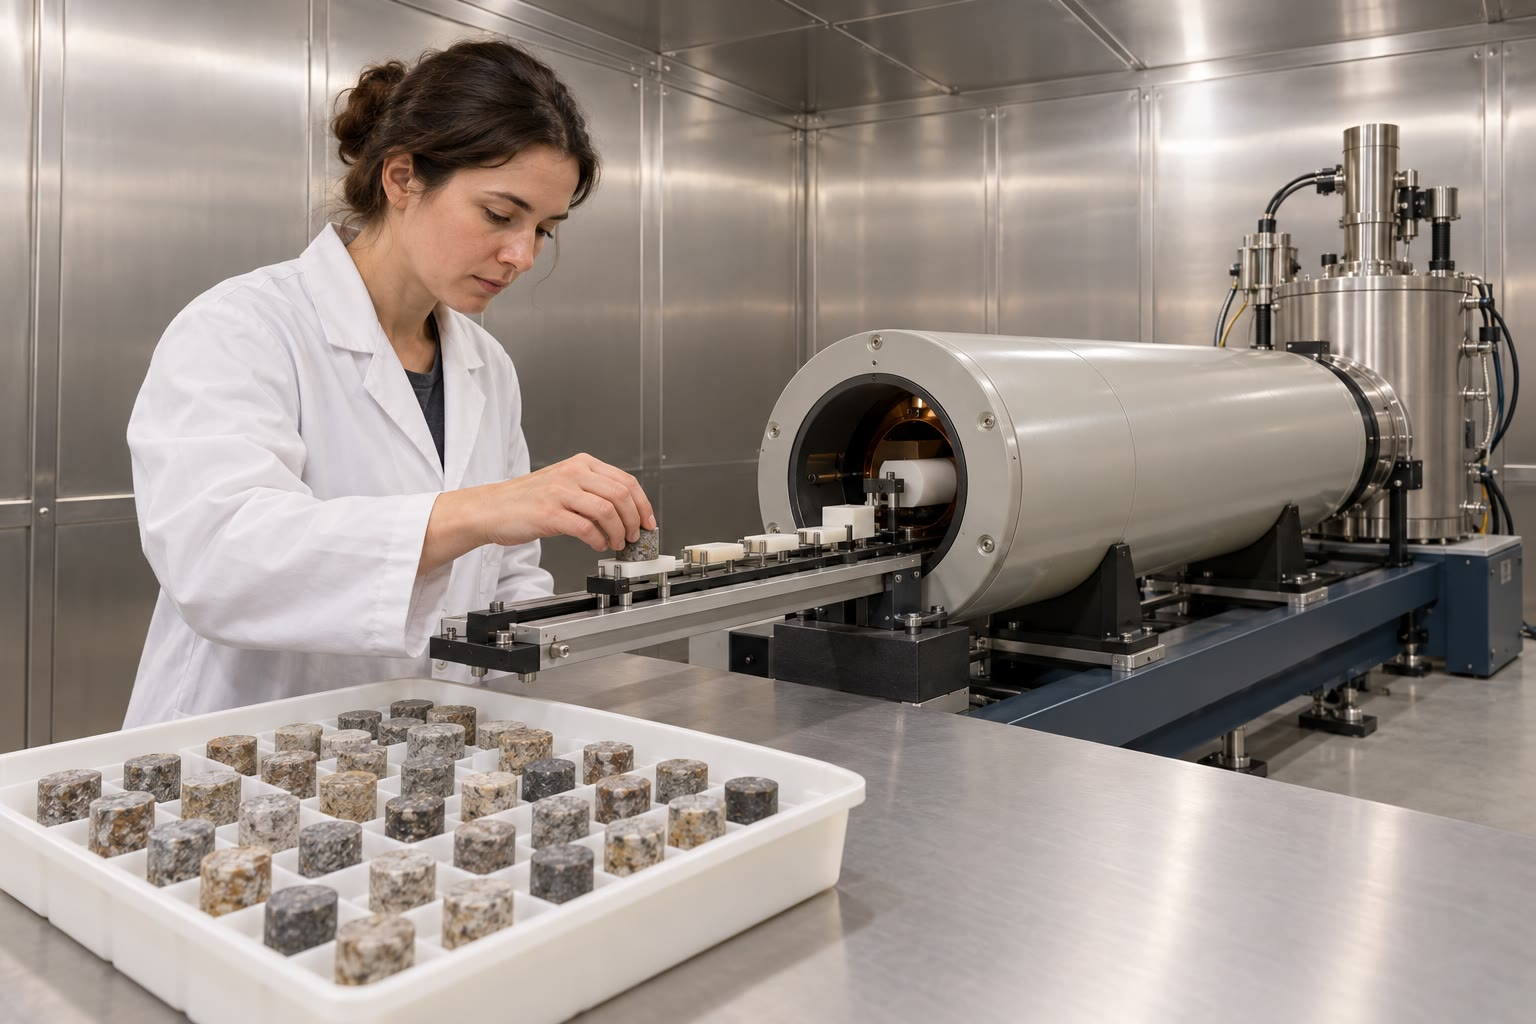
\includegraphics[width=\linewidth]{images/book5/ai/b3-palaeomag-lab.jpg}

{\scriptsize تحميل العيّنات على صينية العيّنات لمقياس المغناطيسية في
غرفة محمية (رسم توضيحي مولَّد بالذكاء الاصطناعي).}
\end{minipage}
\end{inthelab}

\section{التمارين}

\begin{exercise}[$\star$]\label{exo:b3:palaeomagnetism:1}
في حقل \omterm{def:b3:palaeomagnetism:main-field}{ثنائي القطب المحوري المركزي الأرضي}، احسب \omterm{def:b3:palaeomagnetism:inclination}{الميل المغناطيسي} عند خط العرض
\ang{30}\,شمالًا، وخط العرض لموقع يبلغ فيه الميل \ang{-20}.
\end{exercise}

\begin{exercise}[$\star$]\label{exo:b3:palaeomagnetism:2}
عند محطة، للحقل المركّبات $X = \qty{20000}{nT}$، $Y =
\qty{-2000}{nT}$ و$Z = \qty{40000}{nT}$. احسب $H$، $F$، الانحراف المغناطيسي
\omterm{def:b3:palaeomagnetism:inclination}{والميل المغناطيسي}.
\end{exercise}

\begin{exercise}[$\star$]\label{exo:b3:palaeomagnetism:3}
في 2025، $g_1^0 = \qty{-29350}{nT}$. باعتبار الحقل ثنائي قطب محوري،
احسب الحقل عند خط الاستواء وعند القطبين، وعزم ثنائي القطب
($a = \qty{6371.2}{km}$, $\mu_0 = 4\pi\times\qty{e-7}{H.m^{-1}}$).
\end{exercise}

\begin{exercise}[$\star$]\label{exo:b3:palaeomagnetism:4}
سمِّ نوع المغنطة المتبقية المكتسبة، ومتى تسجّل الحقل، في الحالات التالية: (أ) تبرّد تدفّق الحمم؛
(ب) ترسّب الطمي في بحيرة هادئة؛ (ج) حجر رملي تتحوّل فيه طلاءاتُ أكاسيد الحديد
إلى الهيماتيت أثناء الدفن المبكّر؛ (د) بازلت يستقرّ
مدّةَ مليون سنة في الحقل الحالي.
\end{exercise}

\begin{exercise}[$\star\star$]\label{exo:b3:palaeomagnetism:5}
أربع عيّنات من موقعٍ تعطي الاتجاهات $(D, I)$: $(\ang{12}, \ang{48})$،
$(\ang{22}, \ang{44})$، $(\ang{16}, \ang{57})$ و$(\ang{6}, \ang{53})$.
احسب متجهاتها الوحدية، وطول المحصّلة $R$، والاتجاه المتوسط، $k$
و$\alpha_{95}$.
\end{exercise}

\begin{exercise}[$\star\star$]\label{exo:b3:palaeomagnetism:6}
موقع عند \ang{40.0}\,شمالًا، \ang{10.0}\,شرقًا يعطي الاتجاه المتوسط $D = \ang{20}$،
$I = \ang{50}$. احسب خط عرضه القديم وقطبه المغناطيسي الأرضي الافتراضي.
\end{exercise}

\begin{exercise}[$\star\star$]\label{exo:b3:palaeomagnetism:7}
يعطي IGRF عزمَ ثنائي قطب قدره \qty{8.32e22}{A.m^2} في 1900
و\qty{7.69e22}{A.m^2} في 2025، ومعدّل تغيّر $g_1^0$ قدره
\qty{+12.6}{nT/yr} في 2025. (أ) احسب التغيّر النسبي للعزم لكلّ
قرن. (ب) إذا حافظ $g_1^0$ على ذلك المعدّل، فبعد كم سنة يبلغ الصفر؟
لماذا لا يُعدّ هذا تنبّؤًا؟
\end{exercise}

\begin{exercise}[$\star\star$]\label{exo:b3:palaeomagnetism:8}
المغنطة المتبقية للعيّنة، بوحدة \unit{mA/m} (شمالًا، شرقًا، نحو الأسفل)، هي
$(32.2, 18.1, 38.2)$ بعد تسخينها إلى \qty{20}{\celsius}، $(25.8, 18.1, 24.6)$
بعد \qty{300}{\celsius}، و$(0.0, 0.0, 0.0)$ بعد \qty{580}{\celsius}؛ \omterm{def:b3:palaeomagnetism:zijderveld}{ومخطط
زيجدرفيلد} مستقيم بين كلّ زوج. احسب اتجاه
وشدّة المركّبة المُزالة بين 20 و\qty{300}{\celsius}
وتلك المُزالة فوق \qty{300}{\celsius}. أيّهما هي ChRM، وما هي
الأخرى؟
\end{exercise}

\begin{exercise}[$\star\star$]\label{exo:b3:palaeomagnetism:9}
تكوين يعطي $I = \ang{-35}$ مع $\alpha_{95} = \ang{5}$. احسب خط عرضه
القديم، ومدى خطوط العرض القديمة المسموح بها عبر $I \pm \alpha_{95}$،
وأنصاف المحاور $\mathrm dp$ و$\mathrm dm$ لبيضاوي الثقة
الخاص بقطبه.
\end{exercise}

\begin{exercise}[$\star\star\star$]\label{exo:b3:palaeomagnetism:10}
(أ) من \cref{thm:b3:palaeomagnetism:dipole}، أوجد خط العرض الذي يبلغ عنده \omterm{def:b3:palaeomagnetism:inclination}{الميل
المغناطيسي} \ang{45}، ونسبة شدّة المجال عند القطبين إلى شدّته عند
خط الاستواء. (ب) بيّن أنّ $\mathrm dI/\mathrm d\lambda = 2/(1 + 3\sin^2\lambda)$،
واستنتج عند أيّ خط عرض يُعطي خطأ الميل أكبر خطأ
في \omterm{def:b3:palaeomagnetism:vgp}{خط العرض القديم}. (ج) لماذا تكون خطوط العرض القديمة المستنتجة من الميول المنخفضة هي الأكثر
دقّةً بالدرجات؟
\end{exercise}

\begin{exercise}[$\star\star\star$]\label{exo:b3:palaeomagnetism:11}
يقع موقع عند \ang{35.0}\,جنوبًا، \ang{150.0}\,شرقًا على صفيحة مستقرّة، وقطبها المرجعي
لعمر التكوين المأخوذ منه العيّنة هناك، يقع عند \ang{70.0}\,شمالًا،
\ang{300.0}\,شرقًا. (أ) احسب المسافة الزاوية $p$ من الموقع إلى القطب،
والميل المتوقّع والانحراف المتوقّع، \omterm{def:b3:palaeomagnetism:vgp}{وخط العرض القديم} المتوقّع.
(ب) يعطي التكوين $D_o = \ang{30.0}$، $I_o = \ang{-60.0}$. احسب
الدوران $R$ والإزاحة $P$ باتجاه القطب، وبيّن ما يعنيانه.
\end{exercise}

\begin{exercise}[$\star\star\star$]\label{exo:b3:palaeomagnetism:12}
(أ) من \cref{prop:b3:palaeomagnetism:fisher}، بيّن أنّ احتمال أن يقع اتجاه ما
ضمن الزاوية $\theta$ من المتوسط هو $(e^\kappa -
e^{\kappa\cos\theta})/(e^\kappa - e^{-\kappa})$. (ب) عندما تكون $\kappa$ كبيرةً
و$\theta$ صغيرةً، بيّن أنّ هذا يساوي تقريبًا $1 - e^{-\kappa\theta^2/2}$، واستنتج
أنّ \qty{63}{\percent} من الاتجاهات تقع ضمن $\theta_{63} \approx
\ang{81}/\sqrt\kappa$. (ج) احسب $\theta_{63}$ من أجل $\kappa = 50$، وتحقّق من
النسبة \qty{63}{\percent} باستخدام الصيغة الدقيقة.
\end{exercise}

\section{مسألة: الطبقات الحمراء في كيستا}

\begin{problem}[{مسألة نهاية الأسبوع --- ثلاثة تكوينات لرقعة قشرية مُزاحة،
اتجاهاتها وأقطابها ودورانها، وعمر أحدثها}]
\label{pb:b3:palaeomagnetism:1}
% values: calc/ch04.py; palaeomag_stats.py, magnetostratigraphy.py; GPTS: iodp:gpts2004
كيستا رقعة قشرية مُختلَقة، تقع الآن عند \ang{47.0}\,شمالًا، \ang{15.0}\,شرقًا، على حافة
قارّة مستقرّة مُختلَقة. وتكشف ثلاثة تكوينات من الطبقات الحمراء: A،
\qty{60}{Ma}؛ B، \qty{30}{Ma}؛ C، من نحو 3.7 إلى \qty{2.4}{Ma}. وقد أُخذت العيّنات من كلّ تكوين
من عدّة مواقع، وأُزيلت المغنطة حراريًا من كلّ عيّنة؛ \omterm{def:b3:palaeomagnetism:zijderveld}{والمغنطة المتبقية المميِّزة}
ChRM يحملها الهيماتيت، والتكوينات أفقية.

\medskip\noindent\textbf{الجزء الأول --- الاتجاهات المتوسطة.} المواقع الستّة
للتكوين A تعطي $(D, I)$: $(\ang{50}, \ang{37})$، $(\ang{28}, \ang{37})$،
$(\ang{21}, \ang{42})$، $(\ang{24}, \ang{27})$، $(\ang{37}, \ang{39})$،
$(\ang{46}, \ang{38})$.
\begin{enumerate}
  \item لماذا يمكن أن تكون \omterm{def:b3:palaeomagnetism:zijderveld}{المغنطة المتبقية المميِّزة} ChRM التي يحملها الهيماتيت في طبقة حمراء أحدث من
        الطبقة نفسها؟ ما الذي يدلّ على أنّها ليست أحدث بكثير؟
  \item احسب المتجهة الوحدة للاتجاه الأوّل.
  \item مجموع المتجهات الوحدة الستّ يساوي $(3.8943, 2.6500, 3.5717)$. احسب $R$
        والاتجاه المتوسط للتكوين A.
  \item احسب $k$ و$\alpha_{95}$ للتكوين A.
  \item يعطي التكوين B، من 7 مواقع، $D = \ang{23.9}$، $I = \ang{51.5}$
        و$R = 6.8979$؛ والتكوين C، من 8 مواقع، $D = \ang{3.4}$، $I =
        \ang{63.7}$ و$R = 7.8707$. احسب $k$ و$\alpha_{95}$ لكلّ منهما.
  \item أيّ التكوينات أفضل تجميعًا؟ وأيّ المتوسطات أفضل تحديدًا؟
\end{enumerate}

\medskip\noindent\textbf{الجزء الثاني --- خطوط العرض القديمة والأقطاب.}
\begin{enumerate}[resume]
  \item احسب خطوط العرض القديمة للتكوينات A وB وC.
  \item للتكوين A، احسب متمّم \omterm{def:b3:palaeomagnetism:vgp}{خط العرض القديم} $p$ وخط عرض
        قطبه المغناطيسي الأرضي الافتراضي.
  \item احسب خط طول ذلك القطب، متحقّقًا أيّ حالة من
        \cref{thm:b3:palaeomagnetism:pole} تنطبق.
  \item احسب $\mathrm dp$ و$\mathrm dm$ لقطب التكوين A.
  \item يقع قطبا B وC عند \ang{66.5}\,شمالًا، \ang{135.6}\,شرقًا
        و\ang{87.1}\,شمالًا، \ang{139.1}\,شرقًا. صِف مسار الأقطاب الثلاثة
        بتغيّر العمر.
\end{enumerate}

\medskip\noindent\textbf{الجزء الثالث --- عمر التكوين C.} في التكوين C،
من قاعدته، العيّنات ذات قطبية معكوسة حتّى \qty{4.2}{m}، وذات قطبية طبيعية حتّى
\qty{14.8}{m}، ثمّ معكوسة حتّى \qty{19.7}{m}، وطبيعية حتّى \qty{24.6}{m}، ومعكوسة حتّى
\qty{29.2}{m} وطبيعية حتّى \qty{54.0}{m}، ثمّ معكوسة حتّى القمّة عند
\qty{64.0}{m}. طبقة رماد عند \qty{22}{m} مؤرَّخة بنحو \qty{3.2}{Ma}. وتمتدّ الفترات
الطبيعية الفرعية للحقبة C2An على 3.596--3.330، و3.207--3.116،
و3.032--\qty{2.581}{Ma}.
\begin{enumerate}[resume]
  \item طابِق نطاقات القطبية بالمقياس الزمني مستعينًا بطبقة الرماد.
  \item احسب معدّل التراكم بين أوّل حدّ انعكاس للقطبية وثالثه،
        وبين رابعه وسادسه.
  \item قدّر أعمار قاعدة المقطع وقمّته.
  \item لماذا يكون المعدّل متوسّطًا على مدى مئات الآلاف من السنين، وما الذي
        يمكن أن يجعله يتغيّر؟
\end{enumerate}

\medskip\noindent\textbf{الجزء الرابع --- مقارنةً بالقارّة المستقرّة، والانجراف.} الأقطاب المرجعية
للقارّة المستقرّة تقع عند \ang{78.0}\,شمالًا، \ang{190.0}\,شرقًا
($A_{95} = \ang{3.0}$) عند \qty{60}{Ma}؛ \ang{83.5}\,شمالًا، \ang{175.0}\,شرقًا
($\ang{2.5}$) عند \qty{30}{Ma}؛ و\ang{87.5}\,شمالًا، \ang{150.0}\,شرقًا ($\ang{2.0}$)
عند \qty{4}{Ma}.
\begin{enumerate}[resume]
  \item احسب المسافة الزاوية من كيستا إلى القطب المرجعي عند \qty{60}{Ma}،
        والميل المتوقّع \omterm{def:b3:palaeomagnetism:vgp}{وخط العرض القديم} المتوقّع.
  \item احسب الانحراف المتوقّع عند \qty{60}{Ma}.
  \item الاتجاهان المتوقّعان عند 30 و\qty{4}{Ma} هما $(\ang{2.9},
        \ang{60.0})$ و$(\ang{2.5}, \ang{63.6})$. احسب الإزاحة نحو القطب
        $P$ للتكوينات A وB وC.
  \item احسب الدوران $R$ للتكوينات A وB وC.
  \item احسب الخطأين $\Delta D_o$ و$\Delta D_x$ للتكوين A، وخطأ
        دورانه.
  \item أخطاء $R$ للتكوينين B وC هي \ang{13.8} و\ang{17.9}. أيّ الدورانات
        ذات دلالة إحصائية عند 95 في المئة؟
  \item اروِ تاريخ كيستا بالنسبة إلى القارّة المستقرّة.
  \item احسب انجراف كيستا نحو الشمال منذ التكوين A، بالنسبة إلى محور الدوران،
        بالدرجات وبالكيلومترات
        (\qty{111.19}{km} لكلّ درجة).
  \item احسب خطوط العرض القديمة المسموح بها عبر $I \pm \alpha_{95}$ للتكوين
        A، واعتبر الانحراف المعياري نصف عرض تلك
        الفترة مقسومًا على 1.96. وأعطِ انجراف كيستا نحو الشمال منذ التكوين
        A بالكيلومترات، مع انحرافه المعياري.
\end{enumerate}
\end{problem}
